In the study of fluid dynamic systems, the \textit{von Kármán vortex street} phenomenon stands a classical example of pattern formation in flows behind bodies. The pattern is characterized by alternating vortices, and it is not just an example of the complexity of fluid dynamics, but also of great importance in various research fields influencing the design of objects in fluid or aerodynamic systems. For example, the performance of a wing heavily depends on the specific flow, and therefore emergence of vortices can have an impact on the efficiency of the plane and its flight capabilities in various situations. The potential optimization of shape and coatings to achieve desired flight performances led alone in the field of aircraft engineering to a multitude of studies and research activities. Another very interesting occurrence of the phenomenon is shown in \cref{fig: example vortices}, where the interplay of a mountain and wind leads to pattern formation in the clouds and forms alternating vortices. 

\begin{figure}[!htb]
        \centering
        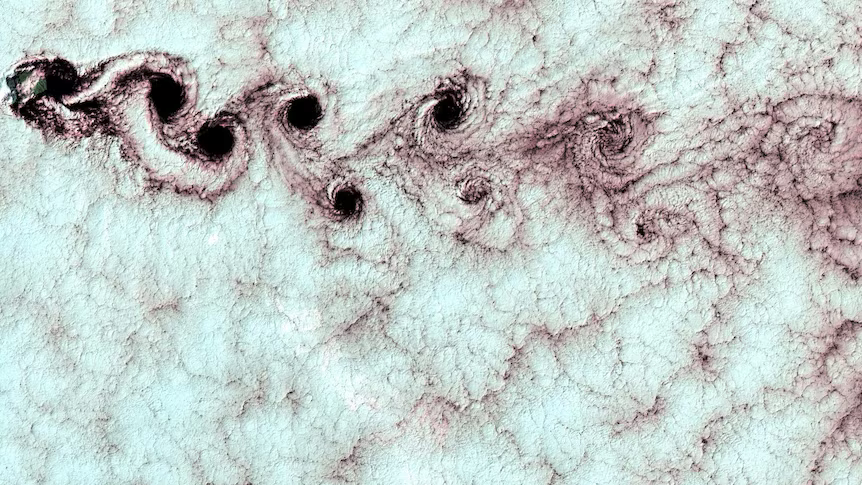
\includegraphics[width=0.6\linewidth]{0_graphics/example_atmos.png}
        \caption{View of a von Kármán vortex street in the atmosphere, showcasing the pattern of swirling vortices caused by airflow around a mountain \cite{wiki}.}
        \label{fig: example vortices}
\end{figure}

This project aims to numerically simulate this phenomenon in a two-dimensional flow field. By leveraging the \textit{Chorin projection method} to decouple the velocity and pressure fields and using a \textit{Semi-Langrangian} solver for the advective term in the underlying equations, we aim to simplify the computational complexity inherent in fluid dynamics problems and to ensure stability and accuracy in the representation of vortex shedding and evolution over time.
Therefore, the plan for the following report is as follows.

First, we introduce the underlying equations as well as the boundary conditions in \cref{sec: posingProblem} that we deal with, and present and motivate the solver in \cref{sec: diffScheme}. In \cref{sec: results}, we numerically simulate the system and investigate the flow patterns for various setups and different shapes.